\documentclass[a4paper,12pt]{article}

\usepackage{polski}
\usepackage[UTF8]{inputenc}
\usepackage{amsmath}
\usepackage[pdftex]{graphicx}
\usepackage[bookmarksnumbered,colorlinks,plainpages,backref]{hyperref}

\hypersetup{
 citecolor=green,
 linkcolor=red,
 filecolor=magenta,
 urlcolor=blue}
\pdfoptionpdfminorversion=7 %Przed dodaniem tej linijki nie chciał przyjąć żadnego obrazka z powodu zbyt wysokiej
\author{Dariusz~Klonowski}  %wersji pdf(1.7).
\title{Matematyczna Przygoda}
\linespread{1.2}
\begin{document}
\maketitle
\tableofcontents
\newpage
\section{Spotkanie pierwszego stopnia z liczbami zespolonymi}
\label{sec:SpotkaniePierwszegoStopniaZLiczbamiZespolonymi}
\subsection{Liczby zespolone - definicja}
\label{subsec:LiczbyZespoloneDefinicja}

Liczbą zespoloną nazywamy liczbę postaci:
\begin{figure}[h]
\centering
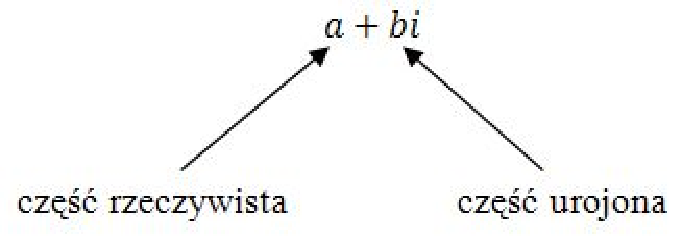
\includegraphics[scale=0.5]{liczba_zespolona.pdf}
\caption{Schemat liczby zespolonej}
\label{fig:liczba1}
\end{figure}

gdzie $a$, $b$ - to dowolne liczby rzeczywiste.

Rysunek \eqref{fig:liczba1} świetnie pokazuje, że jeżeli weźmiemy $b=0$, to otrzymamy zwykłą liczbę rzeczywistą.
Jeżeli natomiast weźmiemy $a=0$, to otrzymamy liczbę zespoloną, która będzie czysto urojona (tzn. nie bedzie mieć części rzeczywistej).

Gdy podajemy część urojoną liczby zespolonej, to ograniczamy się jedynie do współczynnika liczbowego stojącego przy
$i$ (samej jednostki urojonej $i$ nie piszemy).
Liczby zespolone często oznacza się symbolem $z$. Możemy zapisać~np.: $z=7+13i$.
To jest tylko takie umowne oznaczenie, podobnie jak np. liczby naturalne oznaczamy często literką $n$.
Na początku rozdziału pokazaliśmy sobie, że każda liczba zespolona składa się z części rzeczywistej i części urojonej. Teraz to trochę uściślimy i powiemy sobie co dokładnie oznaczają poznane przed chwilą pojęcia.

Przyjmijmy, że mamy daną liczbę zespoloną $z=a+bi$. Wówczas mamy:
\begin{figure}[h]
\centering
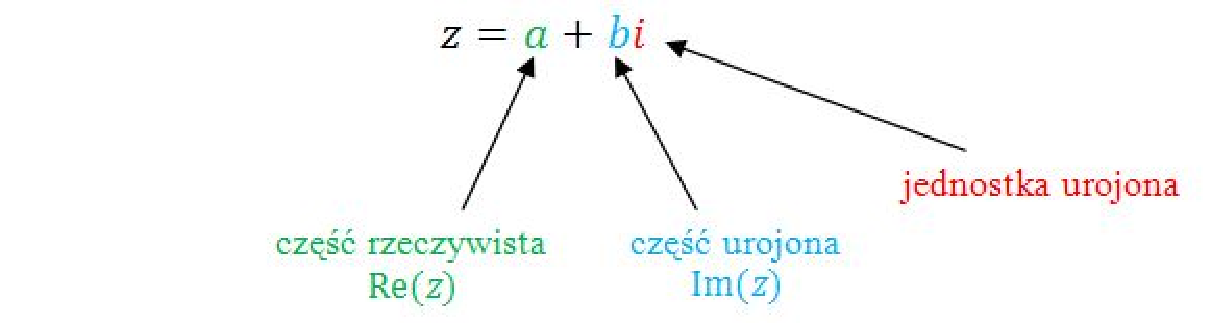
\includegraphics[scale=0.4]{liczba_zespolona2.pdf}
\caption{Schemat liczby zespolonej $z$}
\label{fig:liczba2}
\end{figure}

\begin{flushleft}
\textsf{UWAGA} odnośnie zapisu części rzeczywistej i urojonej.
\end{flushleft}
\begin{itemize}
	\item \texttt{Część rzeczywistą} liczby zespolonej $z$ oznaczamy symbolem: \texttt{Re(z)} (ang. \texttt{Real}).
	\item \texttt{Część urojoną} liczby zespolonej $z$ oznaczamy symbolem: \texttt{Im(z)} (ang. \texttt{Imaginary}).
\end{itemize}
\begin{center}
\textsf{Liczba zespolona jako para liczb rzeczywistych (punkt)}
\end{center}

Wiemy już, że każdą liczbę zespoloną jednoznacznie określają dwie liczby rzeczywiste (część rzeczywista i część urojona). W związku z tym, każdą liczbę zespoloną $z=a+bi$ można utożsamiać z parą liczb rzeczywistych:
\begin{equation}
(a,b)
\label{eq:1}
\end{equation}
\cite{matemaks1}

\subsection{Sprzężenie liczby zespolonej}
\label{subsec:SprzezenieLiczbyZespolonej}
Przyjmijmy, że mamy daną liczbę zespoloną $z=a+bi$.
Wówczas liczbę $a-bi$ nazywamy liczbą sprzężoną do $z$ i oznaczamy symbolem $\overline{z}$.
Czyli:
\begin{equation}
\overline{z} = a - bi
\label{eq:2}
\end{equation}

Dla liczb sprzężonych zachodzą:
\\[0.6 cm]
\begin{tabular}{|l|} \hline
Dla dowolnych $z$, $z_{1}$, $z_{2}$ $\in$ $C$ mamy: \\
~~~~$z+\overline{z}=2Re(z)$ \\
~~~~$\overline{z_{1}+z_{2}}=\overline{z_{1}}+\overline{z_{2}}$ \\
~~~~$z\overline{z}=|z|^{2}$ \\ \hline
\end{tabular}
\\[0.6 cm]
W trzecim podpunkcie pojawił się nowy symbol $|z|$, który oznacza moduł liczby $z$.
Moduł liczby zespolonej $z=a+bi$ liczymy ze wzoru:
\begin{equation}
|z|=\sqrt{a^{2}+b^{2}}
\label{eq:3}
\end{equation}

Pojęcie modułu zostanie wyjaśnione w rozdziale \ref{subsec:ModulLiczbyZespolonej}
\cite{matemaks2}

\subsection{Moduł liczby zespolonej}
\label{subsec:ModulLiczbyZespolonej}
Przyjmijmy, że mamy daną liczbę zespoloną $z=a+bi$.
Wówczas liczbę $sqrt{a^{2}+b^{2}}$ nazywamy \texttt{modułem} liczby $z$ i oznaczamy symbolem $|z|$.
Czyli:
\begin{equation}
|z|=\sqrt{a^{2}+b^{2}}
\label{eq:4}
\end{equation}
Z modułem liczby zespolonej są związane następujące fakty:
\\[0.6 cm]
\begin{tabular}{|l|} \hline
Dla dowolnych $z$, $z_{1}$, $z_{2}$ $\in$ $C$ mamy: \\
~~~~$z\overline{z}=|z|^{2}$ \\
~~~~$|z_{1}\cdot z_{2}|=|z_{1}|\cdot|z_{2}|$ \\
~~~~$|z_{1}+z_{2}|\leq|z_{1}|\cdot|z_{2}|$ \\ \hline
\end{tabular}
\cite{matemaks3}

\subsection{Interpretacja geometryczna liczby zespolonej}
\label{subsec:InterpretacjaGeometrycznaLiczbyZespolonej}
W rozdziale \ref{subsec:LiczbyZespoloneDefinicja} Liczby zespolone - definicja powiedzieliśmy sobie, że każdej liczbie zespolonej $z=a+bi$ odpowiada uporządkowana para liczb $(a, b)$. Przykładowo:
\\[1.1 cm]
\begin{tabular}{|c|c|} \hline
$a+bi$ & $(a,b)$ \\ \hline
$2+5i$ & $(2,5)$ \\ \hline
$5+2i$ & $(5,2)$ \\ \hline
$7-i$ & $(7,-1)$ \\ \hline
$-8-2i$ & $(-8,-2)$ \\ \hline
$i$ & $(0,1)$ \\ \hline
$1$ & $(1,0)$ \\ \hline
$0$ & $(0,0)$ \\ \hline
$12-\sqrt{5}+(7-\sqrt{2})i$ & $(12-\sqrt{5},7-\sqrt{2})$ \\ \hline
\end{tabular}
\\[1.1 cm]
W związku z tym możemy interpretować liczby zespolone jako punkty na płaszczyźnie.
Na osi x będziemy zaznaczać część rzeczywistą liczby zespolonej, a na osi y część urojoną.

Rysunek \ref{fig:liczba3} pokazuje przykładową liczbę zespoloną na płaszczyźnie:

\begin{figure}[ht]
\centering
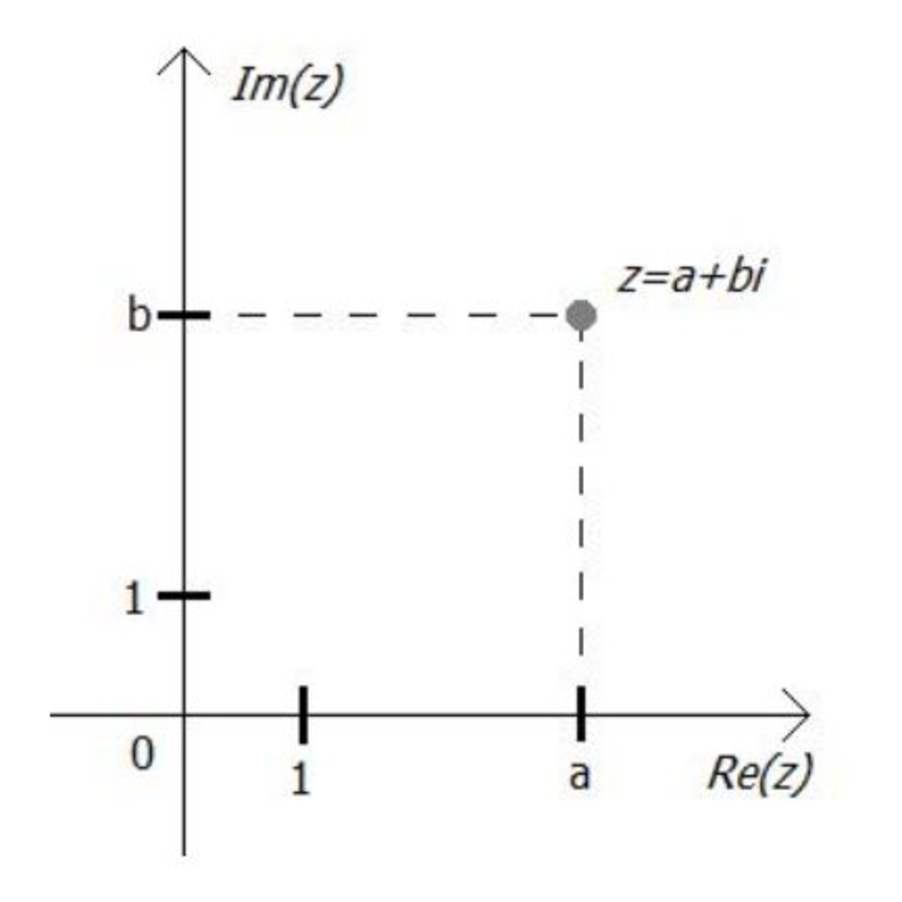
\includegraphics[scale=0.4]{liczba_zespolona3.pdf}
\caption{Interpretacja geometryczna liczby $z$}
\label{fig:liczba3}
\end{figure}

Zaznaczymy teraz jeden ogólny punkt na płaszczyźnie zespolonej i określimy dla niego kilka własności.

\begin{figure}[h]
\centering
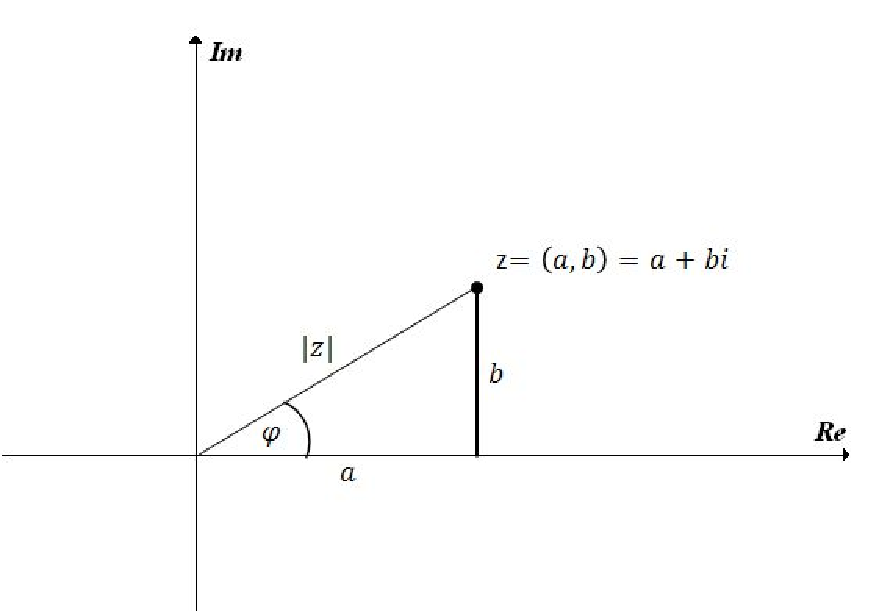
\includegraphics[scale=0.6]{liczba_zespolona4.pdf}
\caption{Liczba $z$ tworzy trójkąt prostokątny}
\label{fig:liczba4}
\end{figure}

Zauważmy na początku, że odległość liczby zespolonej $z=a+bi$ od początku układu współrzędnych, z twierdzenia Pitagorasa, wyraża się wzorem:
\begin{equation}
|z|=\sqrt{a^{2}+b^{2}}
\label{eq:5}
\end{equation}
Czyli jest to po prostu moduł liczby $z$.

Literką $\phi$ (czytamy: fi) oznaczyliśmy kąt między osią Re, a półprostą wychodzącą z początku układu współrzędnych i przechodzącą przez punkt $z$.
Oczywiście nie trzeba obowiązkowo stosować literki $\phi$ na oznaczenie tego kąta. Można posługiwać się dowolną inną literką, np.: $\alpha$, $\beta$, $\gamma$.

Dla ułatwienia przyszłych rachunków miarę zaznaczonego kąta $\phi$ będziemy zazwyczaj wyrażać w radianach (a nie w stopniach). Możemy zatem napisać, że $\phi \in R$.
Liczbę $\phi$ nazywamy argumentem liczby $z$ i oznaczamy $Arg z$.
Dla liczby $z$ którą zaznaczyliśmy w powyższym układzie współrzędnych mamy:
\begin{equation}
Arg z = \phi
\label{eq:6}
\end{equation}
Korzystając wprost z definicji funkcji trygonometrycznych dla trójkąta prostokątnego narysowanego w powyższym
\ref{fig:liczba4} układzie współrzędnych, otrzymujemy:
\begin{equation}
cos \phi = \frac{a}{|z|},~~~~~~~~
sin \phi = \frac{b}{|z|},~~~~~~~~
cos \phi = \frac{a}{\sqrt{a^{2}+b^{2}}},~~~~~~~~
sin \phi = \frac{b}{\sqrt{a^{2}+b^{2}}}.
\label{eq:7}
\end{equation}
Dwa ostatnie wzory otrzymaliśmy z dwóch pierwszych, po prostu podstawiając do nich wzór na moduł. Dla wygody dalej będziemy posługiwali się głównie tymi wzorami po lewej (bo są krótsze w zapisie). Bezpośrednio z nich otrzymujemy, że:
\begin{equation}
a=|z|cos\phi,~~~~~~~~~~~~~~~~~~b=|z|sin\phi.
\label{eq:8}
\end{equation}
Możemy zatem zapisać, że:
\begin{equation}
z=a+bi=|z|cos\phi+(|z|sin\phi)i=|z|(cos\phi+i sin\phi)
\label{eq:9}
\end{equation}
Wzór, który otrzymaliśmy: $z=|z|(cos\phi+i sin\phi)$ to \textbf{postać trygonometryczna} liczby zespolonej $z=a+bi$.

Wiemy już, że możemy przedstawić jedną liczbę zespoloną na trzy różne sposoby:
\begin{itemize}
\item w postaci ogólnej $z=a+bi$,
\item jako punkt $(a, b)$ na płaszczyźnie,
\item  w postaci trygonometrycznej $z=|z|(cos\phi+i sin\phi)$.
\end{itemize}

Każda z nich ma swoje plusy i minusy. Zaletą postaci trygonometrycznej jest to, że umożliwia w łatwy sposób podnoszenie liczb zespolonych do dużych potęg.
\cite{matemaks4}

\subsection{Liczby zespolone w macierzach}
\label{subsec:LiczbyZespoloneWMacierzach}
A teraz, specjalnie dla tych, którzy poszukują mocnych wrażeń:

\textbf{Ćwiczenie 1.} Oblicz wyznacznik $Det A$ macierzy $A$:
\begin{displaymath}
\mathbf{A} =
\left[ \begin{array}{cccc}
15+46i & -27-3i & -7+17i & 87 \\
48-18i & -37+7i & -23-\sqrt{17}i & -18+i \\
-65+5i & -11-7i & 14i & 15 \\
\sqrt{13}+i & 9i & 18 & 79-48i \\
\end{array} \right]
\end{displaymath}
\begin{center}
\textsc{{\huge Powodzenia!!! ;-)}}
\end{center}
\begin{figure}[h]
\centering
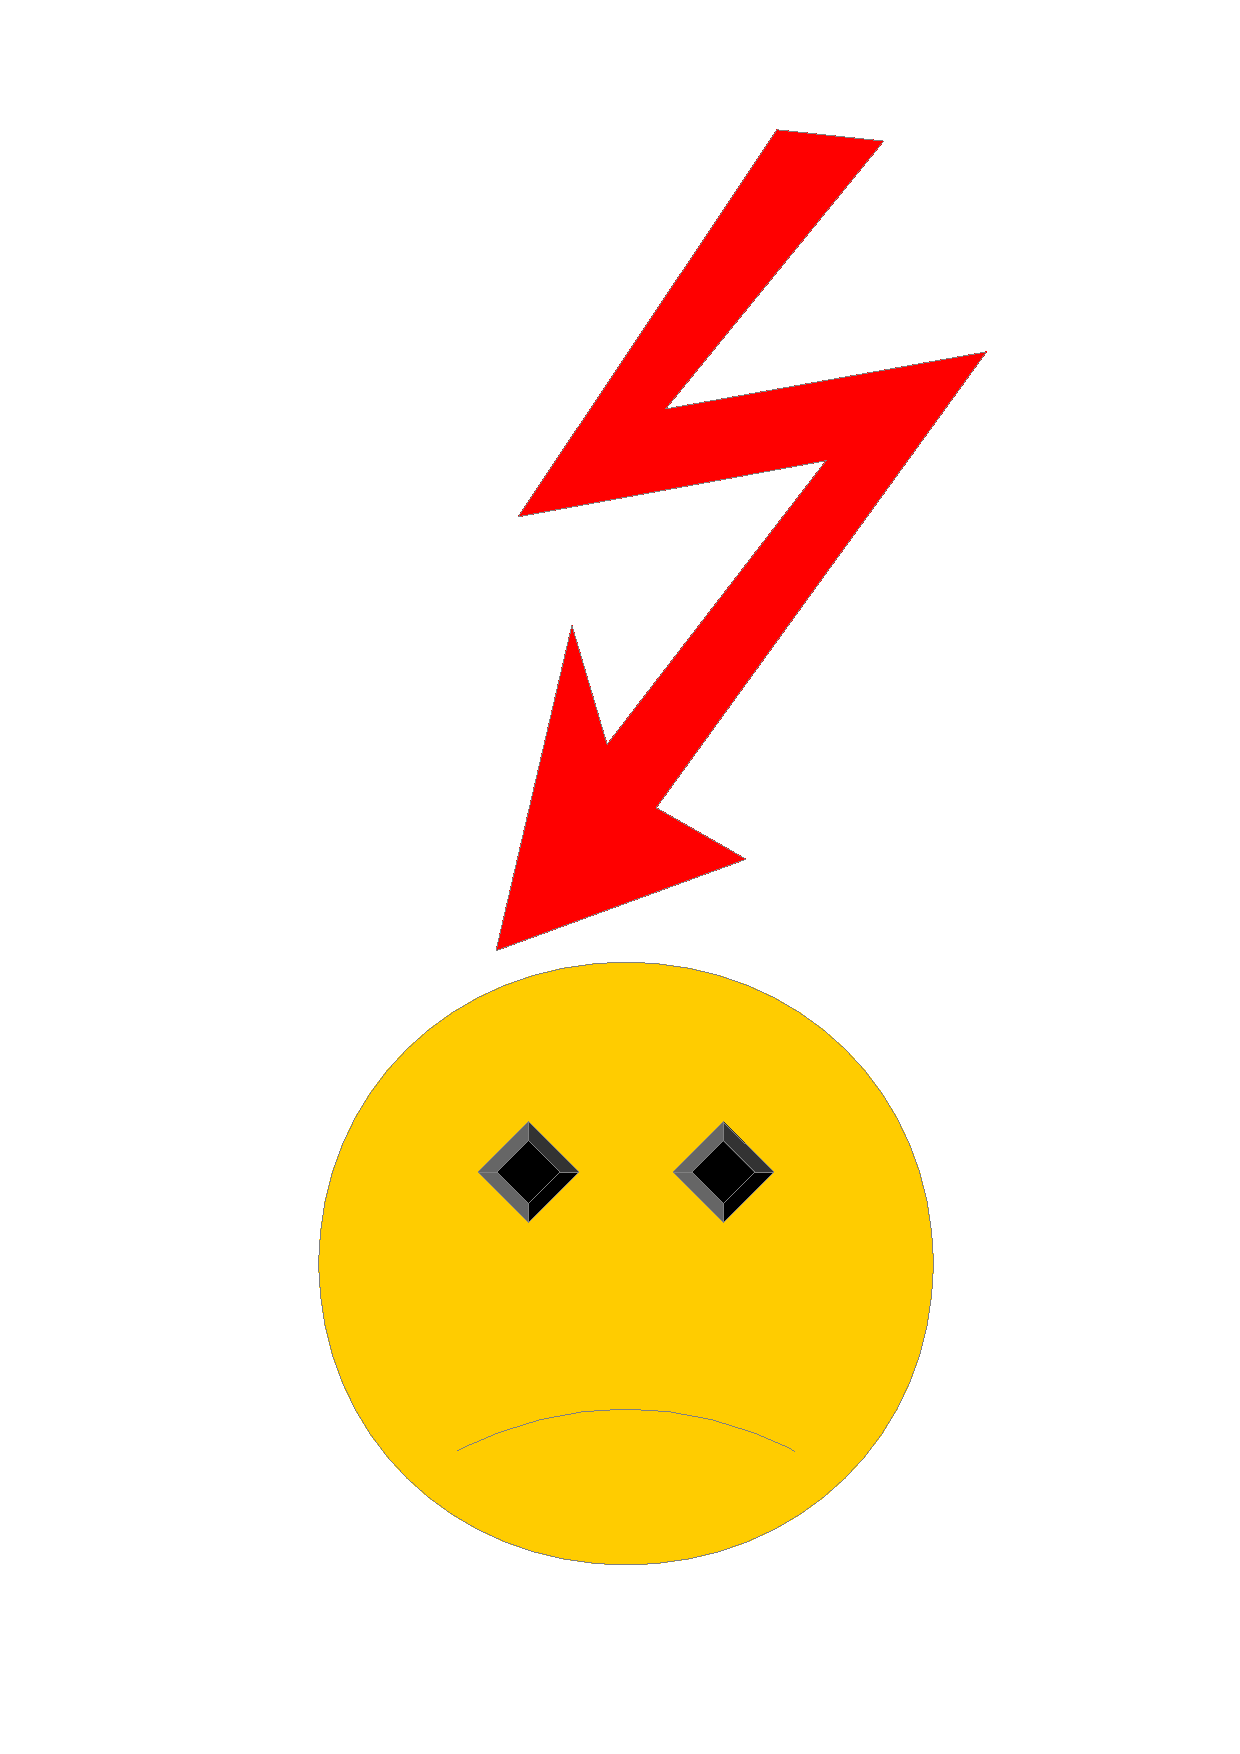
\includegraphics[scale=0.25]{buzka.pdf}
\caption{Tak wygląda czacha po nauce matematyki...}
\label{fig:buzka}
\end{figure}
\newpage
\section{Po ciężkiej pracy (czyt. nauce matymatyki) należy się nieco relaksu\ldots}
\label{sec:PoCiezkiejPracyNalezySieNiecoRelaksu}
\subsection{Kilka żartów \ldots}
\label{subsec:KilkaZartow}
\begin{enumerate}
\item \begin{flushleft}
\begin{verse}
Pewien informatyk poszedł na ryby. \\
Złapał złotą rybkę, która obiecała spełnić tradycyjnie trzy życzenia. \\
Informatyk mówi: \\
- Żeby był pokój na świecie. \\
- Za trudne. \\
- No to, aby Windows się nie zacinał. \\
- To już niech będzie ten pokój na świecie\ldots \\
\end{verse}
\end{flushleft}
\cite{kawal1}

\item \begin{flushleft}
\begin{verse}
Żona do męża informatyka: \\
- Poznajesz człowieka na fotografii? \\
- Tak. \\
- Ok, dzisiaj o 15 odbierzesz go z przedszkola. \\
\end{verse}
\end{flushleft}
\cite{kawal2}

\item \begin{flushleft}
\begin{verse}
Jak informatyk wywiesza pranie? \\
- Na linkach. \\
\end{verse}
\end{flushleft}
\cite{kawal3}

\item \begin{flushleft}
\begin{verse}
- Czym różni się doświadczony informatyk od początkującego? \\
- Początkujący uważa, że 1 KB to 1000 B, a doświadczony jest pewien, że 1 km to 1024 m. \\
\end{verse}
\end{flushleft}
\cite{kawal4}

\item \begin{flushleft}
\begin{verse}
Informatyk do informatyka: \\
- Pożycz mi 500 zł. Albo nie, 512 dla równego rachunku. \\
\end{verse}
\end{flushleft}
\cite{kawal5}

\item \begin{flushleft}
\begin{verse}
Jaki rozmiar piersi powinna mieć żona informatyka? \\
C++. \\
\end{verse}
\end{flushleft}
\end{enumerate}
\cite{kawal6}

\newpage
\section{Podziękowania}
\label{sec:Podziekowania}
{\Large Dziękuję za przeczytanie i zachęcam do pozytywnej oceny mojej
pracy\footnote{Zdanie \emph{"zachęcam do pozytywnej oceny mojej pracy"} należy uznać za skrzywienie zawodowe, ponieważ pracuję w infolinii sieci \texttt{PLAY} i muszę namawiać do niej klientów.}!!! Mam nadzieję, że się podobało ;-)}

\bibliographystyle{plain}
\bibliography{bib}

\end{document} 